\section{Scene and object recognition with Computer Vision}

\subsection{Laparoscopic tool detection}

\begin{center}
\begin{figure}[H]
\centering
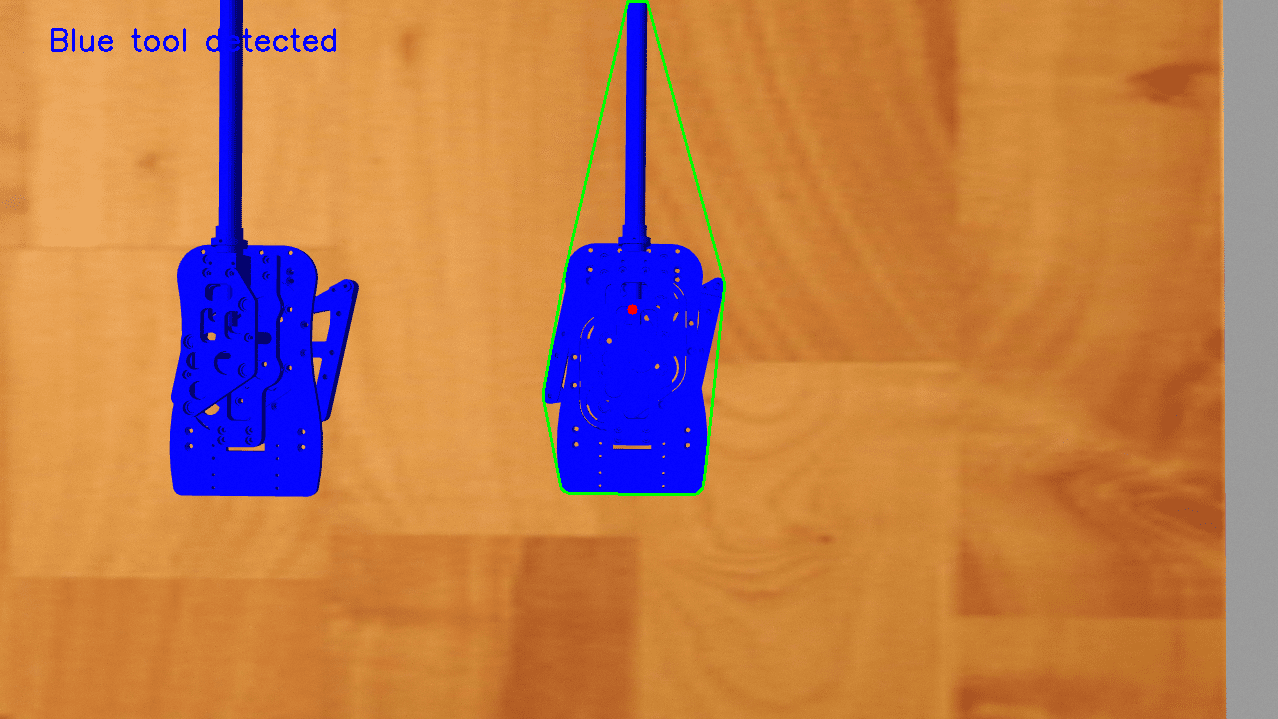
\includegraphics[width=12cm]{images/opencv-tool-convex-hull.png}\\
\caption{Simple tool detection in simulation based on color, using OpenCV. The green polygon is the convex hull, and the red point is the
estimated center of mass}
\end{figure}
\end{center}

\subsection{Calculation of tool position and orientation}

In order for the gripper to grasp correctly the laparoscopic tool, it is required to calculate the tool's position and orientation in the pixel space 
which must then be converted with respect to the robot's workspace. From all the pixels that have been classified as part of the laparoscopic tool, 
one can estimate the center of mass and two perpendicular vectors 
attached to that point that define the orientation. The center of mass is simply the average of the $(x,y)$ coordinates of all the tool's pixels
\[
\left( \bar{x}, \bar{y} \right) = \left( \frac{1}{N}\sum_{i=1}^{N} x_i , \frac{1}{N}\sum_{i=1}^{N} y_i \right)
\]
The two orientation vectors are the eigenvectors of the covariance matrix of the above pixels. Let $\mathbf{a},\mathbf{b}$ be the orientation vectors, 
then $\mathbf{a},\mathbf{b}$ are solutions of the equation
\[
C \mathbf{v} = λ \mathbf{v}
\]
where $C$ is the covariance matrix given by
\[
C = \begin{bmatrix}
σ(x,x) & σ(x,y) \\
σ(y,x) & σ(y,y) \\
\end{bmatrix}
\]
\[
σ(x,y) = \frac{1}{n-1} \sum_{i=1}^{N} ( x_i - \bar{x} )( y_i - \bar{y} )
\]

\begin{center}
\begin{figure}[H]
\centering
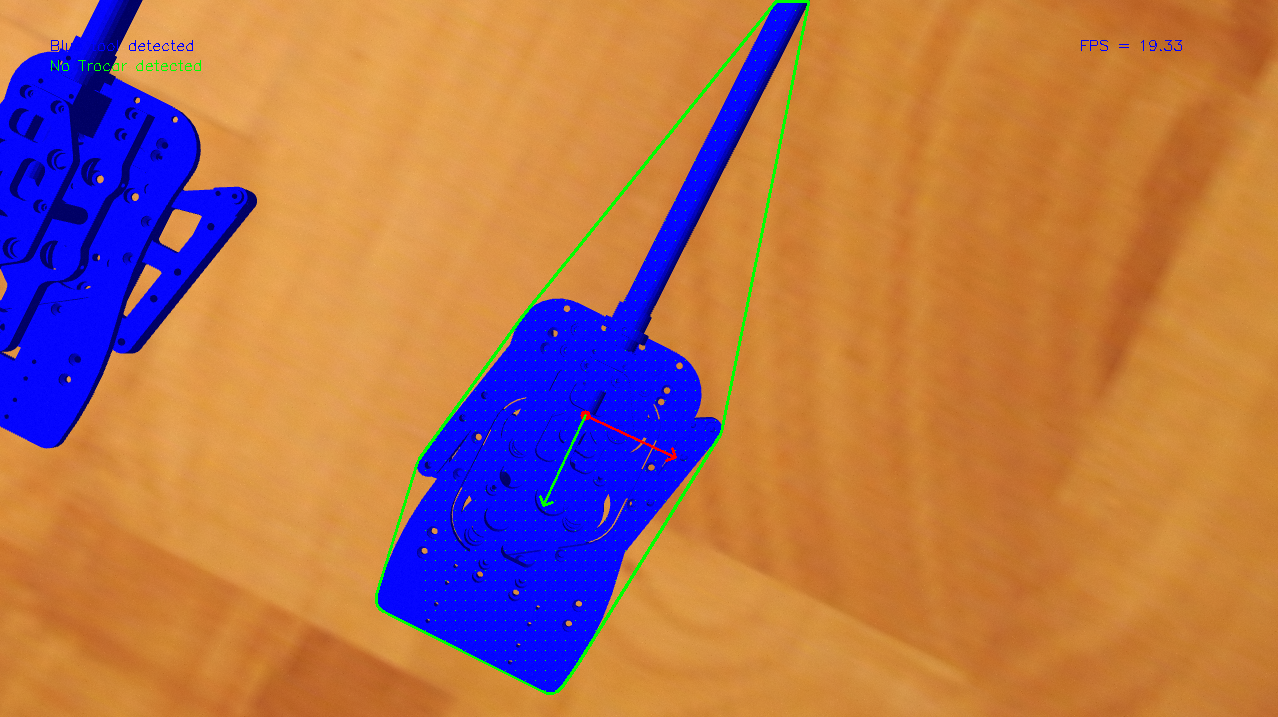
\includegraphics[width=12cm]{images/tool-pose.png}\\
\caption{Estimation of tool's pose (position and orientation)}
\end{figure}
\end{center}

\subsection{Calculation of grasping points}

\subsection{Trocar detection \& Estimation of fulcrum point}

\begin{center}
\begin{figure}[H]
\centering
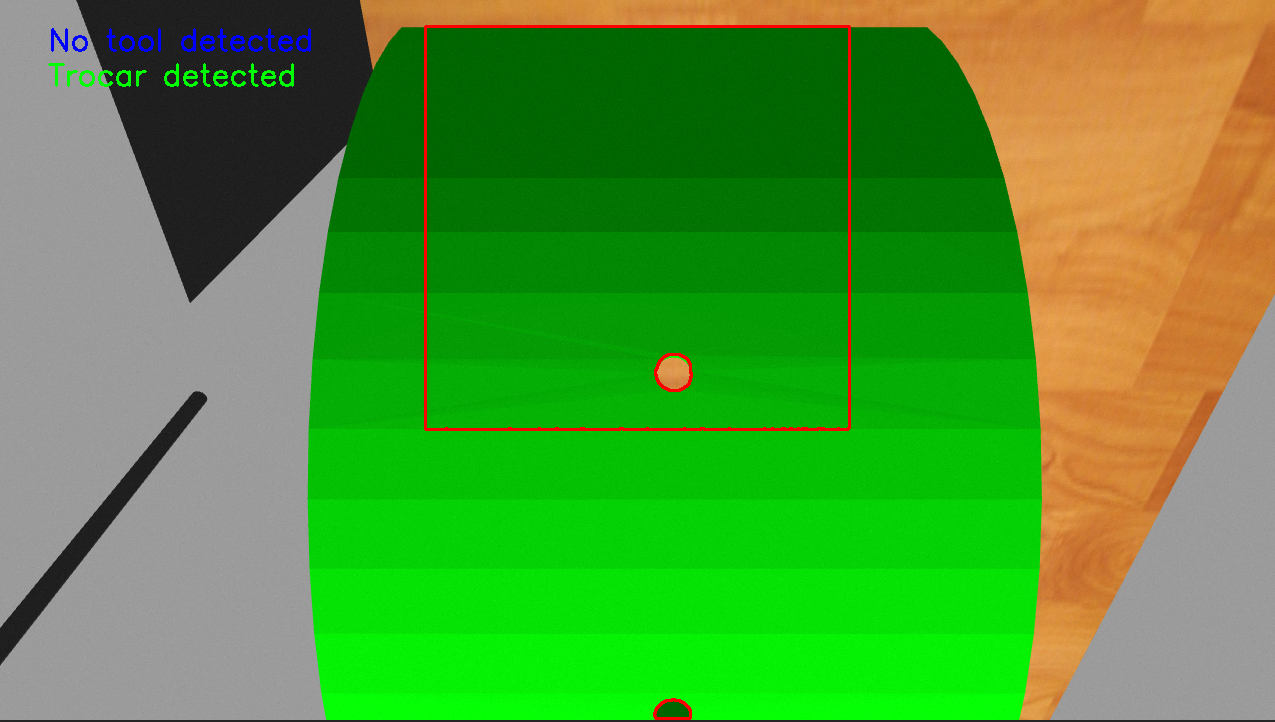
\includegraphics[width=12cm]{images/opencv-trocar-detection.png}\\
\caption{Simple trocar detection in simulation based on color, using OpenCV. In simulation, the trocar is simply considered to be a small 
cylindrical hole and it's center is the fulcrum point}
\end{figure}
\end{center}